%--------------------------------------------------------------------------
% 	NEW SUBSECTION
%--------------------------------------------------------------------------
\section{Simulation vs schematic}
\subsection{Simulation setup}

\begin{frame}
	\tableofcontents[currentsubsection]
\end{frame}

\begin{frame}
\frametitle{Analysis}
	Developed analysis:
	\begin{itemize}
		\item Time domain output mixed signal and spectral components;
			\item Oscillator signal amplitude to maximize output component;
		\item Conversion gain and 1dB compression point;
		\item Single tone IIP\textsubscript{3};
		\item Two tone IIP\textsubscript{3};
		\item Bandwidth and CMRR of RF stage (output node filtering of output signal, current mixing);
		\item Static power dissipation;
	\end{itemize}
	Used frequencies: f\textsubscript{LO}=110MHz, f\textsubscript{RF}=100MHz, with expected f\textsubscript{IF}=10MHz.
\end{frame}

\begin{frame}
	\frametitle{Simulation setup}
	\begin{figure}[H]
		\centering %se si cambia posizione a questa immagine assicurarsi che sia girata con il fondo verso il bordo esterno della pagina
		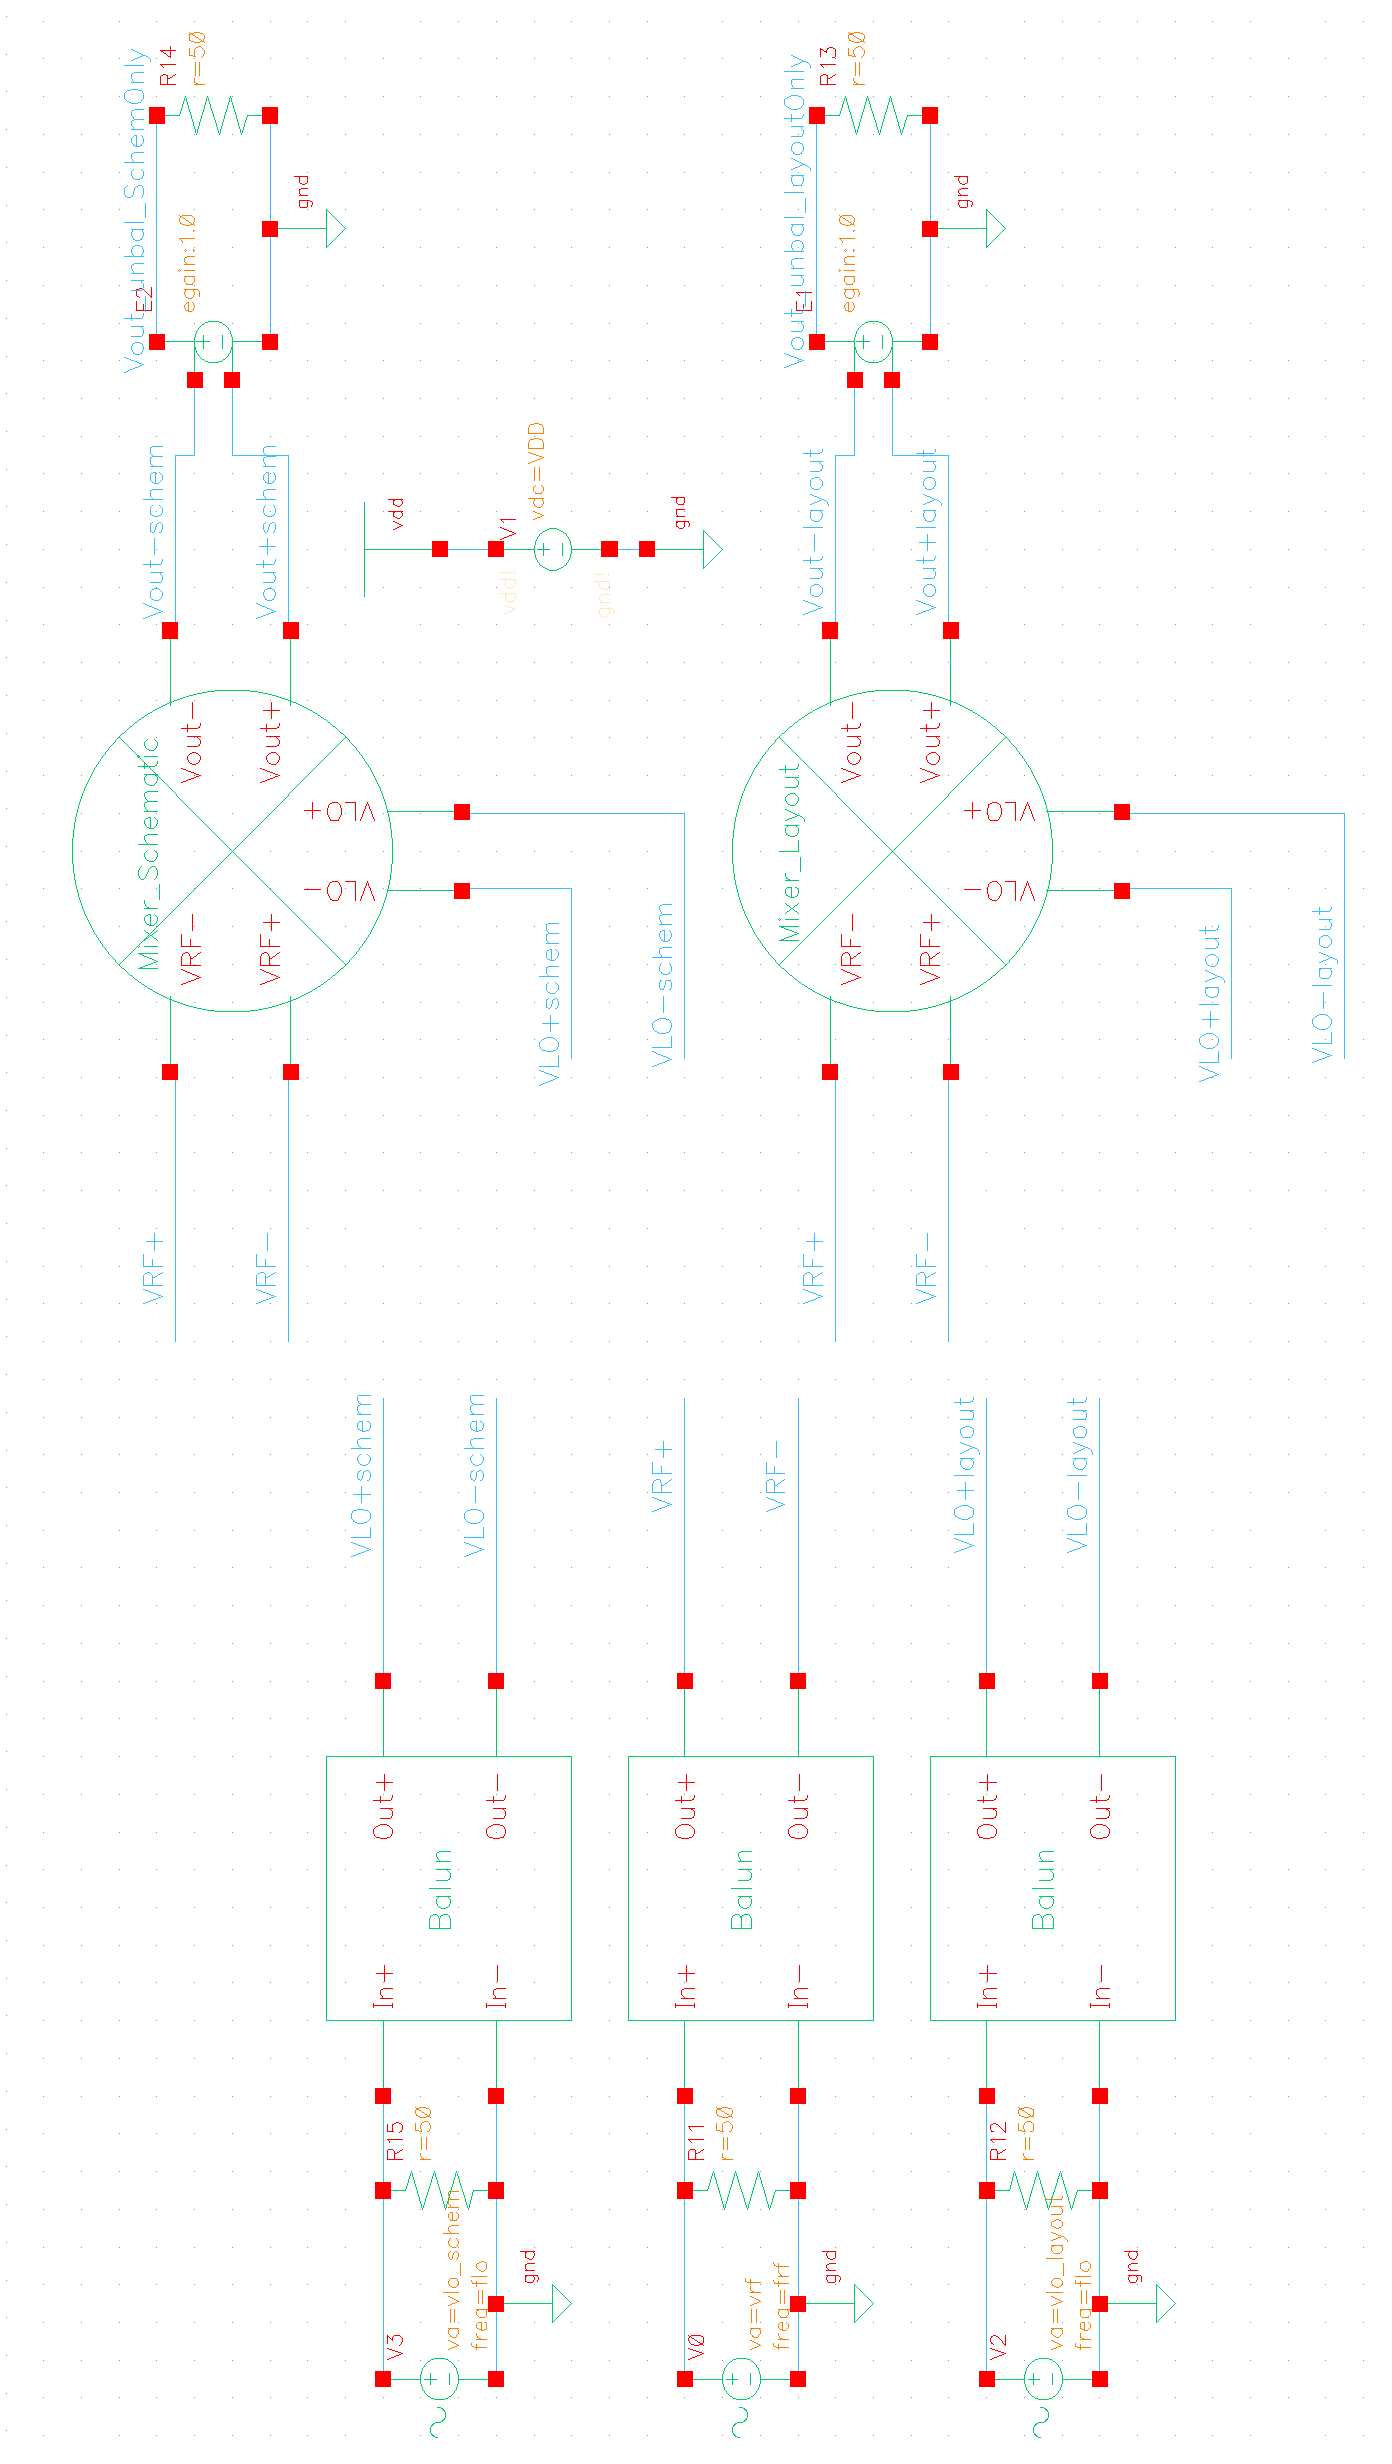
\includegraphics[scale=0.18, angle=-90]{setup}
		\label{fig:setup}
	\end{figure}
\end{frame}

\begin{frame}
	\frametitle{Simulation setup}
	\begin{figure}[H]
		\centering
		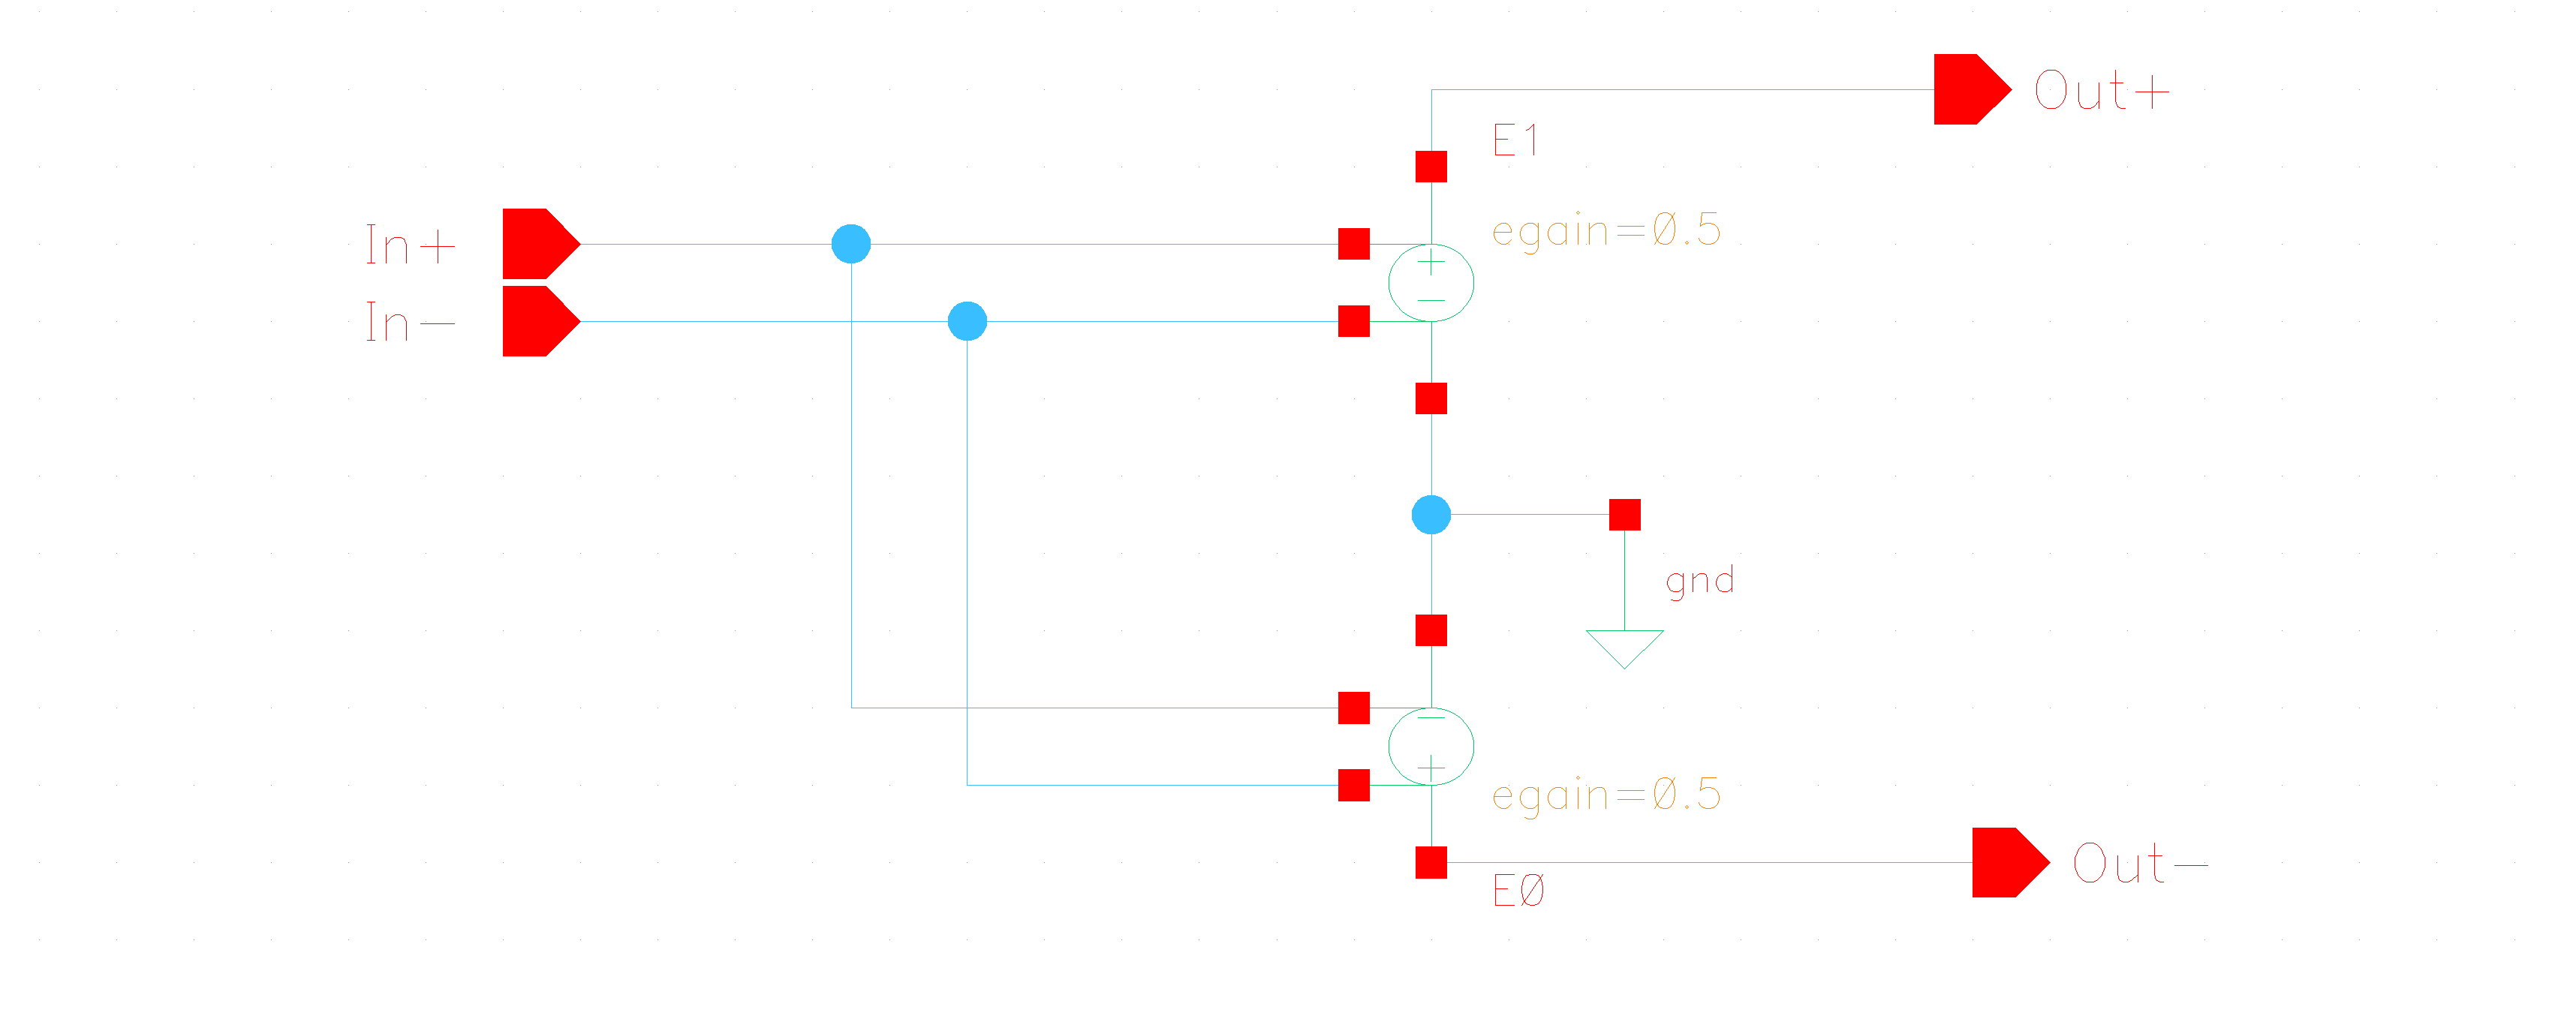
\includegraphics[scale=0.05]{balun}
		\caption{Balun schematic.}
		\label{fig:balun}
	\end{figure}
	\begin{itemize}
		\item Ideal baluns simulate a  50 \(\Omega\) impedance matching condition and produce differential inputs. 
		\item Power supply net, implicitly connected to both layout and schematic.
		\item Mixer's loads, represented by 50\(\Omega\) resistors connected to unitary gain driven generator. Used both for ideal impedance matching purposes and to convert differential output from mixers to single-ended.
	\end{itemize}
\end{frame}

%--------------------------------------------------------------------------
% 	NEW SUBSECTION
%--------------------------------------------------------------------------
\subsection{Time and frequency domain analysis}
\begin{frame}
\tableofcontents[currentsubsection]
\end{frame}

\begin{frame}
	\frametitle{Bandwidth evaluation - Transition frequency}
	Dynamic analysis is complex when dealing with non-linear circuits. The following results try to qualify the circuit in the best way.
	Always monochromatic signals have been used. 
\end{frame}

\begin{frame}
	\frametitle{Bandwidth evaluation - Transition frequency}
	\begin{columns}
	\column{0.4\textwidth}
	Maximum working frequency must be at least one decade below MOSFET transition frequency f\textsubscript{T}.
	From current gain measurements on M\textsubscript{3} and M\textsubscript{6}:
	\begin{gather}
		f_T|_{RF}=9.43GHz \notag \\
		f_T|_{LO}=1.12GHz \notag 
	\end{gather}  
	\column{0.6\textwidth}
	\begin{figure}[H]
		\centering 
		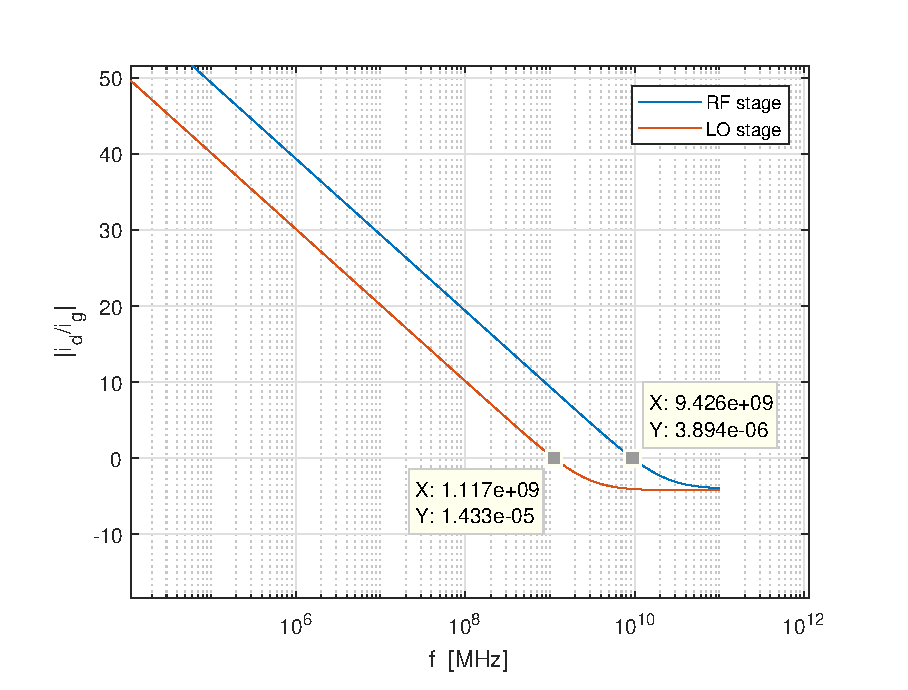
\includegraphics[scale=0.5]{transition_freq}
		\label{fig:ft}
	\end{figure}
	\end{columns}
\end{frame}

\begin{frame}
\frametitle{Bandwidth evaluation - Transition frequency}
\begin{columns}
	\column{0.4\textwidth}
	Bandwidth evaluated by plotting conversion gain dependency on frequency.
	The simulation is performed keeping \(f_{LO}=f_{RF}-10\)MHz.
	-3dB point is located almost two octaves above the maximum operation frequency.
	
	\column{0.6\textwidth}
	\begin{figure}[H]
		\centering 
		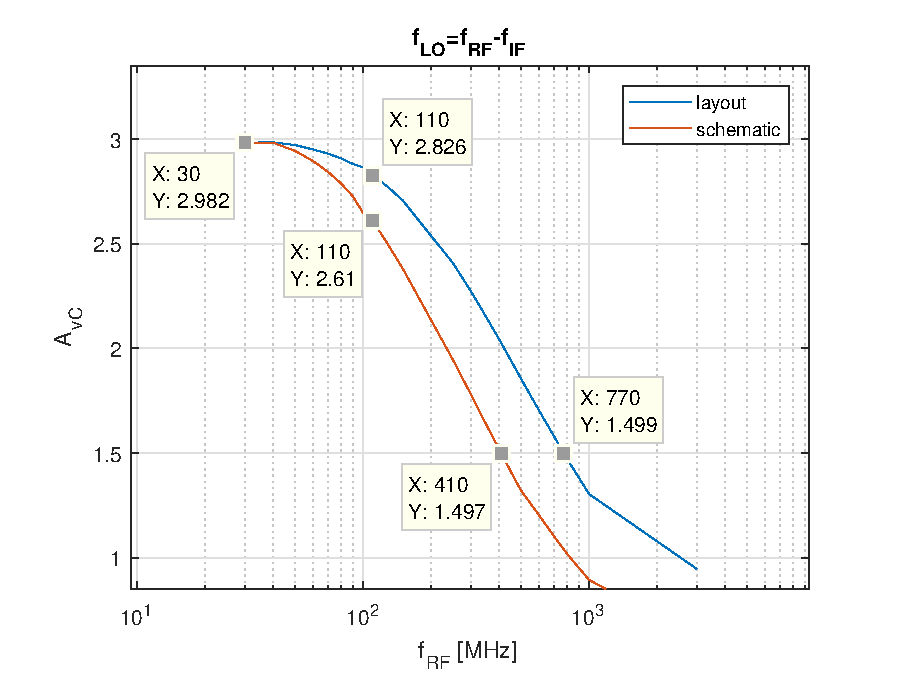
\includegraphics[scale=0.5]{bandwidth}
		\label{fig:band}
	\end{figure}
\end{columns}
\end{frame}

\begin{frame}
	\frametitle{Bandwidth evaluation - Conclusions}
	It is important to notice that we \textbf{cannot rely on this results} because:
	\begin{itemize}
		\item The technology kit is probably not suited for RF operation;
		\item The layout extraction does not account for all device and circuit parasitics, that would affect the performances at high frequency. The physical implementation would  probably not work;
		\item Pretending that results are accurate the simulation emulate the worst case operative condition. 
	\end{itemize}
\end{frame}

\begin{frame}
\frametitle{Max gain vs LO}
\begin{columns}
	\column{0.4\textwidth}
	LO level must be optimized to get maximum conversion gain. RF power is kept constant, sweeping pump input power.
	
	Layout seems to have better performance than schematic in term of maximum gain. From simulation:
	\begin{align}
	&V_{LO,opt}|_{layout}=1.23V \notag \\
	&V_{LO,opt}|_{schematic}=2.5V \notag
	\end{align}
	\column{0.6\textwidth}
	\begin{figure}[H]
		\centering
		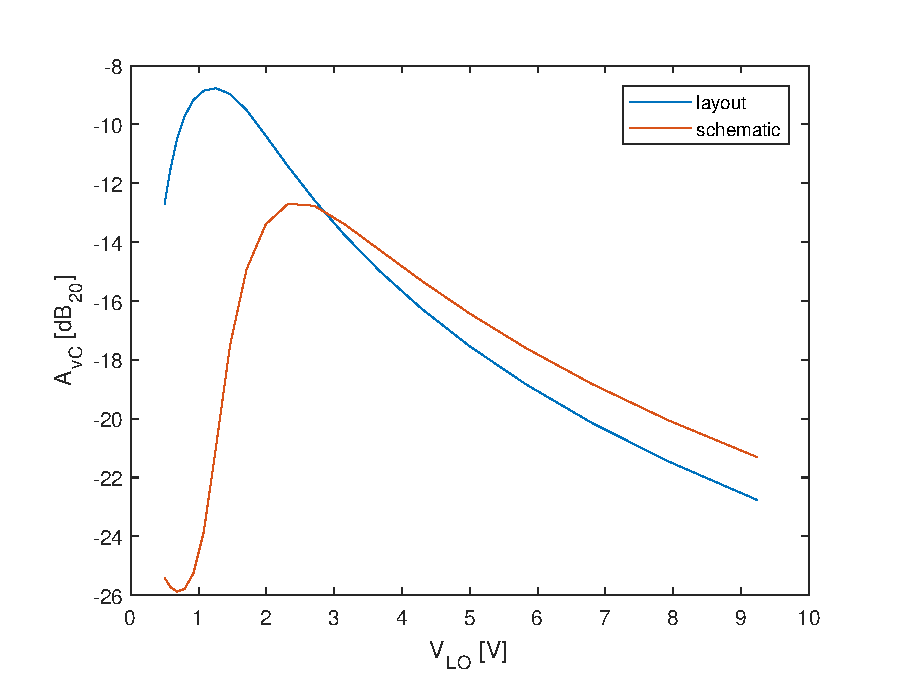
\includegraphics[scale=0.5]{gain_vs_VLO}
		\label{fig:maxGainvsLO}
	\end{figure}
\end{columns}
\end{frame}

\begin{frame}
\frametitle{Time domain analysis}
\begin{columns}
	\column{0.4\textwidth}
	It is possible to have a qualitative analysis about the distortion introduced by the circuit (detailed treatise later), by looking at the dft of the mixer's output signal. 
	\column{0.6\textwidth}
	\begin{figure}[H]
		\centering
		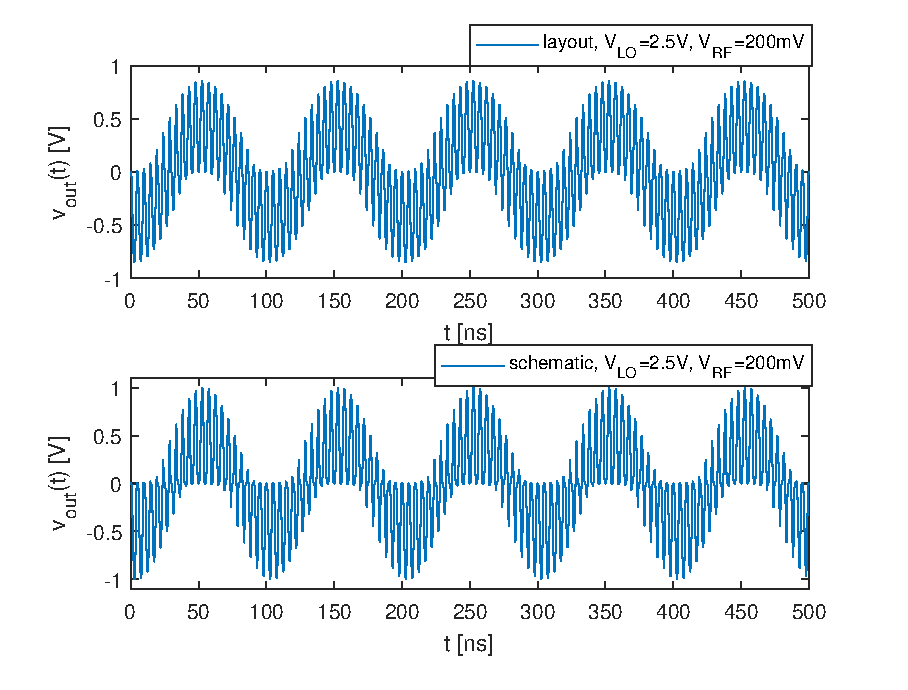
\includegraphics[scale=0.4]{waveforms}
		\caption{Time domain waveforms: double balanced differential output with v\textsubscript{RF}=200mV,  f\textsubscript{RF}=110MHz, v\textsubscript{RF}=1.23mV, f\textsubscript{LO}=100MHz.}
		\label{fig:TdomaniWF}
	\end{figure}
\end{columns}
\end{frame}

\begin{frame}
\frametitle{Output signal spectrum}
	\begin{figure}[H]
		\centering
		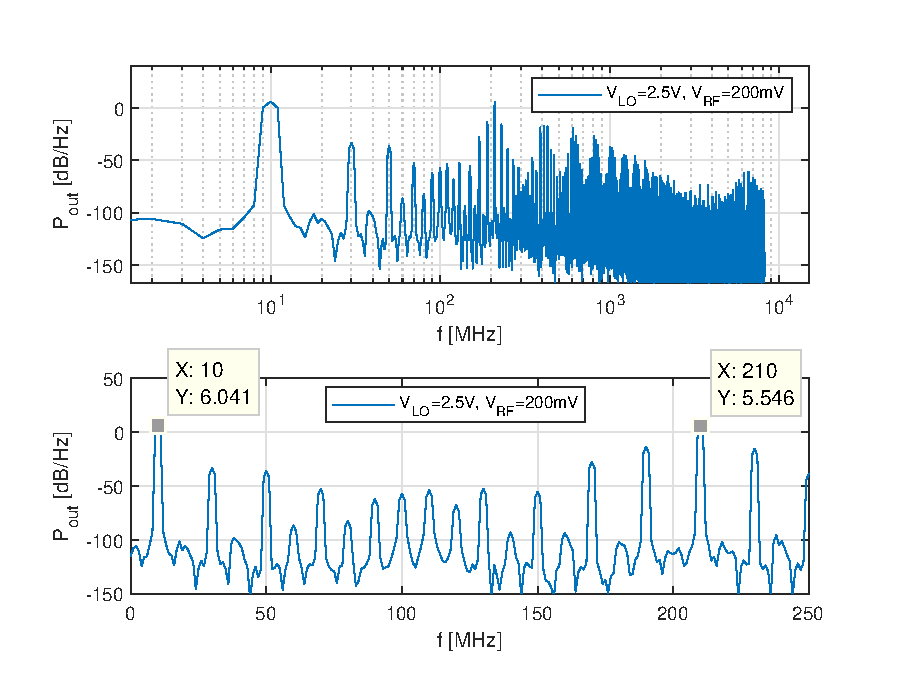
\includegraphics[scale=0.5]{DFT_layout}
		\caption{\textbf{Layout}. Discrete Fourier transform: double balanced differential output with v\textsubscript{RF}=200mV,  f\textsubscript{RF}=110MHz, v\textsubscript{RF}=1.23mV, f\textsubscript{LO}=100MHz,cosine squared smoothing function.}
	\end{figure}
\end{frame}

\begin{frame}
\frametitle{Output signal spectrum}
	\begin{figure}[H]
	\centering
	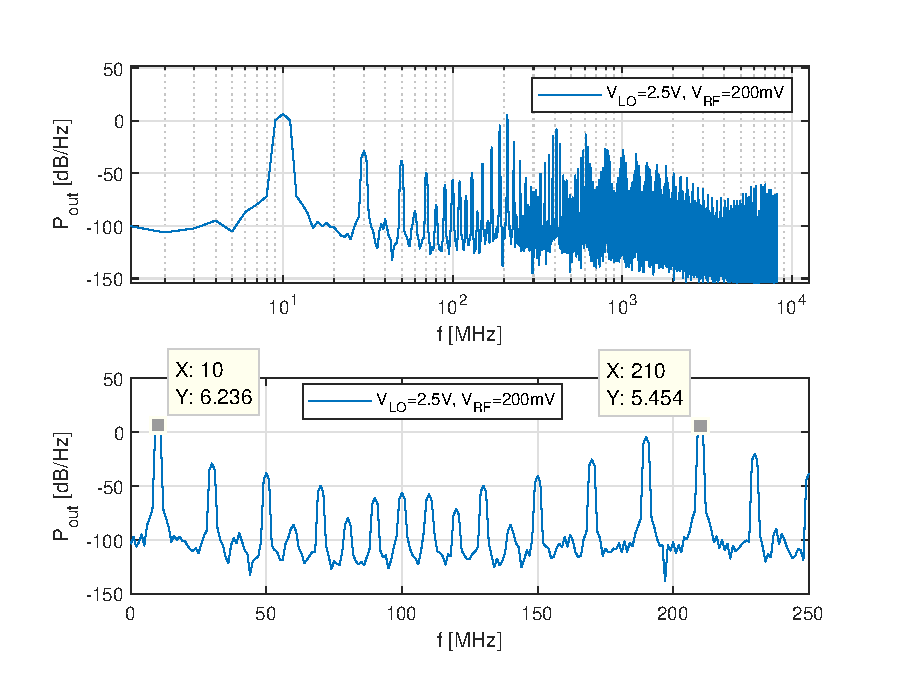
\includegraphics[scale=0.5]{DFT_schem}
	\caption{\textbf{Schematic}. Discrete Fourier transform: double balanced differential output with v\textsubscript{RF}=200mV,  f\textsubscript{RF}=110MHz, v\textsubscript{RF}=1.23mV, f\textsubscript{LO}=100MHz,cosine squared smoothing function.}
	\end{figure}
\end{frame}

